\documentclass[12pt]{texMemo}  
\usepackage[english]{babel}
\usepackage{graphicx, blindtext, setspace, amsmath, amssymb, natbib}
\memoto{Adrienne Davis, Vice Provost}
\memofrom{Jacob M. Montgomery}
\memosubject{The Status of Women in the Political Methodology Subfield}
\memodate{\today}

\usepackage{booktabs}
\begin{document}

\newcommand{\stcomp}[1]{{#1}^\complement}

{\begin{center}
\Large\bf
M\textsc{emorandum}
\end{center}}



\maketitle
\singlespacing

\section*{Introduction: Background}

Political methodology is a subfield of political science focused on research methodology and design, data collection, measurement, statistics, and empirical modeling.
\begin{itemize}\setlength\itemsep{0em}
\item Political methods not exist until the mid 1970s and the first meeting of Society for Political Methodology (SPM) occurred in 1983.  
\item Political methodology has expanded significantly as quantitative approaches to research have increasingly dominated the discipline.  
\item While small in absolute numbers, the quantitative turn in the discipline has made it influential (e.g. \textit{Political Analysis}, the journal of SPM, has been among the top five most influential journals in political science in nine of the last ten years and had the \textit{highest} impact factors in four of the last ten years). 
\end{itemize}

\noindent However, even from its earliest days the methods subfield has struggled to diversify.\footnote{Methods has also struggled extremely with including persons of color -- especially under represented minorities.  However, the focus of this memo is on the status of women.}  
\begin{itemize}\setlength\itemsep{0em}
\item Early meetings of the SPM were almost exclusively male. 
\item While progress has been made, the field still lags far behind the broader discipline. 
\item Like other STEM fields, political methodology struggles to recruit women graduate students and suffers from a ``leaky pipeline.'' 
\end{itemize}
 The net consequence is that political methods is \textbf{the least diverse subfield in all of political science}. 


\section*{Women in political methodology}

\subsubsection*{Our search pool and our program}

Members of the search committee spent considerable time and effort recruiting applicants with special attention paid to identifying women and under-represented minorities.  Nonetheless, only 12 out of the 73 applicants (16.4\%) were women.  The comparable numbers for our searches last year in American politics and comparative politics were  28\% and  24\% respectively. The poor numbers in our pool are not an aberration.  Rather, they are a symptom of a very serious gender representation problem in the methods field.  

This lack of representation contrasts starkly with our own graduate program. Of the 11 women graduate students active in our program, seven (63.6\%) have expressed an interest in the methods field.  Roughly half of the overall methods students in the program are women.  Thus, we are confronted with a situation where:\setlength\itemsep{0em}
\begin{enumerate}
\item our program would benefit from having more descriptive representation of women in the methods field and additional faculty in general to help mentor and train; and
\item women are extremely under-represented in our potential hiring pool.
\end{enumerate}



\subsubsection*{APSA organized section}

The American Political Science Association (APSA) reports that 36.7\% of its members are women.  However, it is clear that women are very unevenly distributed across subfields.  Figure 1 shows the percent of women in 43 of APSA's organized sections.
From this data it is evident that political methodology is an outlier (19.2\% women).
\begin{figure}[h!]
\caption{Percent of women for APSA organized sections}
\vspace{-.5in}
\begin{center}
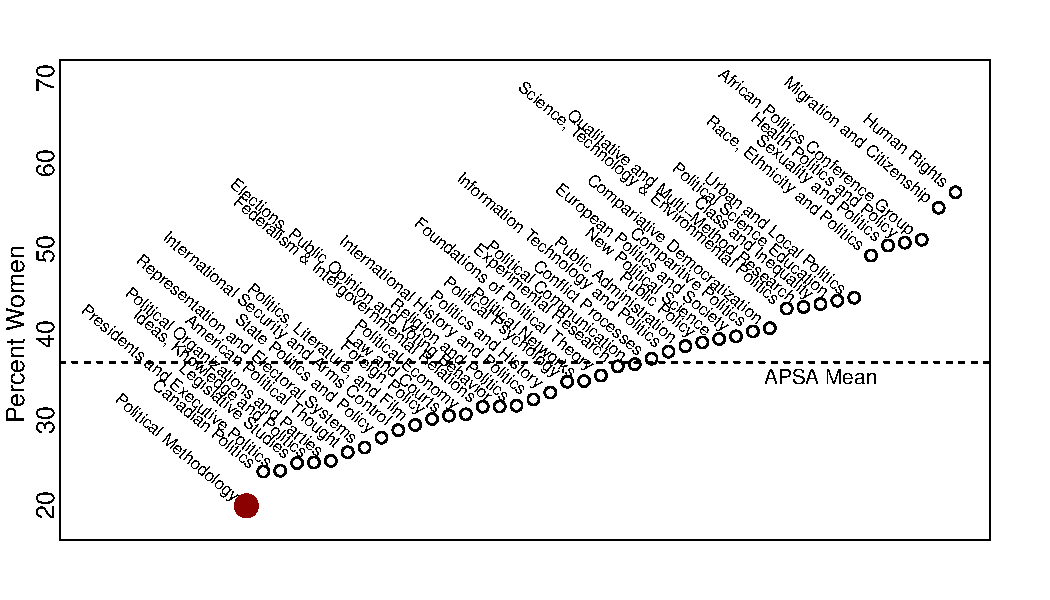
\includegraphics[scale=.85]{sections}
\end{center}

\vspace{-1cm}
\footnotesize Data comes from American Political Science Association.  The Women and Politics Research section (91.6\% women) is excluded from this plot to make it visually clearer. The dashed horizontal line shows the overall percent of women in APSA. 
\end{figure}

\newpage

\subsubsection*{APSA conference participation}

Another way to examine the representation of women in the field is to look at conference participation. I coded the gender of all participants at APSA's 2017 annual meeting who were on a political methodology panel.  The results, shown in Figure 2, indicate that \textbf{only 19\% of methods panelists at our discipline's most prestigious conference were women}.
\vspace{-.6cm}
\begin{figure}[htbp]
\caption{Gender breakdown of APSA 2017 Methods Panels}

\begin{center}
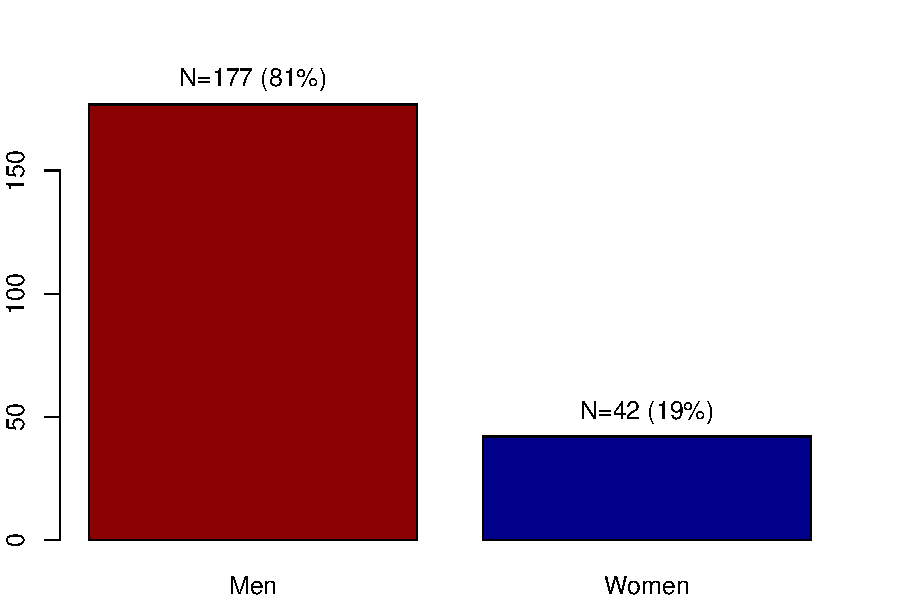
\includegraphics[scale=.5]{apsaGender}
\end{center}


\footnotesize Data collected from the 2017 APSA online program.
\end{figure}
\vspace{-.2in}


\subsubsection*{SPM summer meeting}

The annual summer meeting of the SPM plays a crucial role in defining the political methods field and its membership.  At the 2017 SPM meeting, 57 out of 211 participants were women (27\%).  These numbers are actually obscure worse gender representation issues.   
\begin{itemize} \setlength\itemsep{0em}
\item Only 21.4\% of participants on tenure track jobs were women.   
\item Only 13.8\% of individuals who presented or discussed research in one of the panels were women.
\item  Only 13\% of tenure-track faculty who presented posters were women.
\end{itemize}

\newpage

\begin{figure}[htbp]
\caption{Gender breakdown of 2017 SPM conference by status/participation }
\vspace{-.3in}
\begin{center}
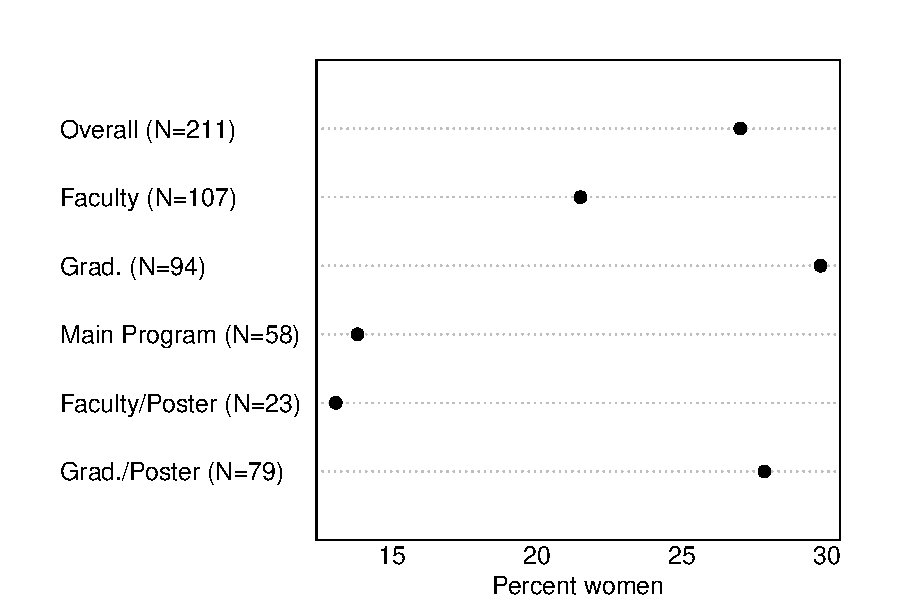
\includegraphics[scale=.8]{polmeth}
\end{center}


\footnotesize Data provided by SPM and coded from the 2017 program.
\end{figure}


\subsubsection*{Limited progress}

The \textit{National Science Foundation} has provided extensive support to SPM to improve representation of women and minorities in the field.  Past efforts have included:
\begin{itemize}\setlength\itemsep{0em}
\item Financial support for targeted groups to attend the annual meeting.
\item A separate conference, Visions in Methodology, designed to mentor and support women entering the methods field.
\item Trial interventions designed to encourage more participation for targeted groups.
\end{itemize}
Despite these efforts, limited progress has been made.  As is shown in the figure below, participation of women has gone up (somewhat) over time. However, participation in 2017 is not appreciably different than it was in 2006 or 2008.

\begin{figure}[htbp]
\caption{Gender breakdown of SPM meeting 2006-2016}
\vspace{-.3in}
\begin{center}
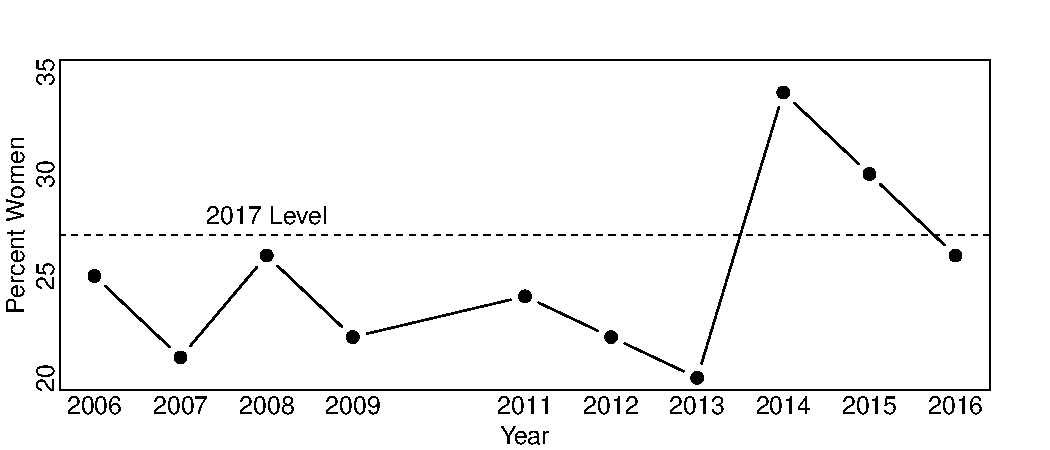
\includegraphics[scale=.9]{overTime}
\end{center}
\end{figure}


\newpage

\subsubsection*{Tenured women methodologists}

As stark as the numbers above are, I will close by pointing out that they are even worse at more senior levels. I am aware of only 13 tenured women in the political methodology field (using a very broad definition) and only eight full professors.\footnote{Janet Box-Steffensmeir (Ohio State), Suzanna Linn (Penn State), Wendy Tam Cho (Illinois), Lonna Atkeson (New Mexico), Betsy Sinclair (WUSTL), Rocio Titiunik (Michigan), Vera Troeger (Warwick), Xun Pang (Tsinghua University), Sunshine Hillygus (Duke), Sarah Mitchell (Iowa), Jennifer Victor (George Mason), Amber Boydston (UC-Davis), Becky Morton (NYU) } At top-25 departments (as ranked by the US News and World Report) there are only seven tenured faculty and only four full professors. 




\end{document}